\documentclass[notes=hide,yellow]{beamer}

% (c) 2008 Steffen Klemer <moh AT gmx BEEP org>
% This work is licensed under the Creative Commons Attribution-Share Alike 3.0
% Germany License. To view a copy of this license, visit
% http://creativecommons.org/licenses/by-sa/3.0/de/ or send a letter to Creative
% Commons, 171 Second Street, Suite 300, San Francisco, California, 94105, USA.
%
% See http://www.noch-mehr-davon.de/vortr.shtml
% Permissions beyond the scope of this license may be available at the same site
%
% Template based on: Copyright 2004 by Till Tantau <tantau@users.sourceforge.net>.


\mode<presentation>
{
%	\usetheme{AnnArbor} %Szeged
%	\usetheme{Berkeley}
	\usetheme{Frankfurt}
%	\usecolortheme{rose} %oder beaver oder rose oder orchid, albatross, rose
% 	\useinnertheme{circles}
%	\useoutertheme{split}
%	\setbeamercovered{invisible} %or transparent
% 	\usefottheme{professionalfonts}
% 	\usefonttheme[onlymath]{serif}
        %\setbeamercovered{invisible}
%	\setbeamertemplate{navigation symbols}{}
}

\usepackage{amsmath,amssymb,latexsym}
\usepackage{fancyvrb}
\usepackage{graphicx}
\usepackage{epstopdf}
\usepackage{amsfonts}
\usepackage{amsthm}
\usepackage{wasysym}
\usepackage{ucs}
\usepackage{listings}
\usepackage{stmaryrd}
\usepackage{hyperref}
\usepackage{graphics}
\usepackage{colortbl}

\usepackage{tikz}
\tikzstyle{every picture}+=[remember picture]
\usetikzlibrary{arrows}
\usetikzlibrary{shadows}
\usetikzlibrary{fit}
\usetikzlibrary{shapes}
\usetikzlibrary{backgrounds}

\tikzstyle{vertex}=[circle,fill=black!25,minimum size=12pt,inner sep=0pt]
\tikzstyle{selected vertex} = [vertex, fill=red!24]
\tikzstyle{blue selected vertex} = [vertex, fill=blue!25]
\tikzstyle{edge} = [draw,thick,-]
\tikzstyle{weight} = [font=\small]
\tikzstyle{selected edge} = [draw,line width=5pt,-,red!50]
\tikzstyle{ignored edge} = [draw,line width=5pt,-,black!20]
\tikzstyle{small vertex}=[circle,fill=black!25,minimum size=8pt, inner sep=0pt]
\tikzstyle{small selected vertex}=[circle,fill=red!25,minimum size=8pt, inner sep=0pt]



%\usepackage[ngerman]{babel}
%\usepackage[utf8x]{inputenc}




\title{An overview of current BGP security problems}
\subtitle{ }
\author{Ralph Krimmel}



\begin{document}
	\begin{frame}
		\titlepage
	\end{frame}

	\begin{frame}
		\tableofcontents
	\end{frame}

\section{ Introduction}
\subsection*{}

\begin{frame}{Routing in the Internet}
\end{frame}

\begin{frame}
	\frametitle{BGP}
\end{frame}

\begin{frame}
	\frametitle{Autonomous Systems}

\end{frame}

\begin{frame}
	\frametitle{Importance of BGP in the Internet}
\end{frame}

\section{Security issues of BGP}
\subsection*{}
\begin{frame}
	\frametitle{Prefix hijacking}
		
	\begin{block}{No verification of:}
		\begin{itemize}
			\item Prefix ownership
			\item AS number ownership
		\end{itemize}
	\end{block}
\end{frame}

\begin{frame}{Short AS pathes}
	\begin{center}
		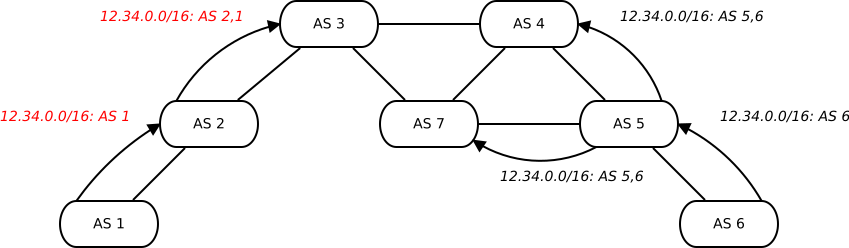
\includegraphics[width=\textwidth]{pathlength.pdf}
	\end{center}
\end{frame}

\begin{frame}{Deaggregation}
	\begin{center}
		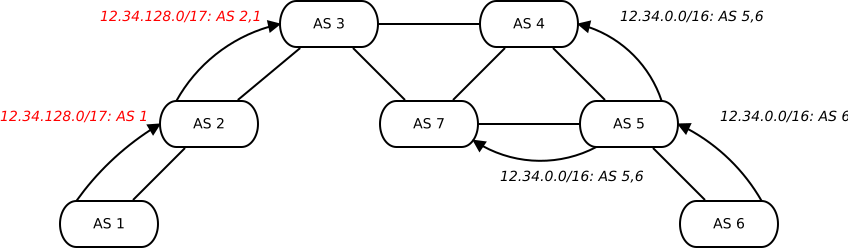
\includegraphics[width=\textwidth]{deaggregation.pdf}
	\end{center}
\end{frame}

\begin{frame}
	\frametitle{Attacks on TCP}
	
	\begin{block}{Attacks on TCP}
	\begin{itemize}
		\item eavesdropping to learn routing information (not a BGP specific attack)
		\item MITM (attacks against integrity
		\item inserting, modifying deleting messages, replay attack
		\item DoS attack against TCP
		\item (sending RST, SYN-Flood, backhoe attack (cutting a link)
	\end{itemize}
	\end{block}

\end{frame}


\begin{frame}
	\frametitle{Attack on the routing policy}
	%Exploiting as path length and MED to manipulate route selection by an AS
\end{frame}

\section{Cryptographic techniques}
\subsection*{}
\begin{frame}{Cryptographig techniques}
\begin{itemize}
	\item Pairwise keying
	\item Cryptographic hash functions
	\item MACs
	\item PKI
	\item Certificates
\end{itemize}
\end{frame}

\section{BGP security today}
\subsection*{}
%target: byzantine robustness
\begin{frame}
	Current approaches: 
	\begin{itemize}
		\item Protection of the BGP sesseion between routers
		\item Defensive filtering
	\end{itemize}
\end{frame}

\section{Session defense}

\begin{frame}
	\frametitle{Protection of a BGP Session between routers}
	2 goals: Protecting TCP and BGP session itself
\end{frame}


\begin{frame}
	\frametitle{Proposed solutions}
	\begin{block}{Countermeasures}
	\begin{itemize}
		\item MD5 Integrity
		\item Session and Message Protection
		\item Generalized TTL Securiy Mechanism
		\item IPsec
	\end{itemize}
	\end{block}

\end{frame}


\begin{frame}{MD5 Integrity}
	
%MD5 integrity: Utilize TCP extension that uses a MAC based on MD5
%-> Protects integrity and prevents replay attacks
%
\end{frame}

\begin{frame}{Session and Message Protection}
%5 Proposed countermeasures:
%Adding sequence numbers
%Encryption of all BGP data between peers (shared secret)
%
%Adding UPDATE sequence numbers/timestamp
%New path attribute: PREDECESSOR: identification of last AS before destination
%digital signatures of all UPDATE fields
%Disadvantages: BGP needs to be altered
%Based on shared secrets => hard to manage huge number of keypairs
\end{frame}

\begin{frame}{Generalized TTL Security Mechanism}
	Utilizing IP TTL to discard every packet with TTL < MAX-1.
	V%=> Weakly defends against remote attacker, but not against malicious information coming from adjacent peers
	%=> Also, useless in multihop environments
\end{frame}

\begin{frame}{IPsec}
%Use IPsec to secure BGP at IP layer
%IKE for key management, AH and ESP for packet level security
%Typically used to secure messages between peers
%Provides: authenticy, integrity, replay prevention, confidentality, DOS prevention
\end{frame}

\section{Defensive Filtering}
\subsection*{}
%Goal: Filter bad and potential malicious announcmentce
%Usually ingress and egress filtering based on route policies like:
%prefixes with special uses
%bogons/martians (advertisements of adress blocks and AS numbers with no matching allocation data)
%=> filtering using an updated list of bogons
%filter out private AS numbers
%too long AS-Pathes
%routes to small soubnets (snm > 24)
%hard limit of announcments by a neighbour
%filtering by customer policies
%Rewrite of BGP attributes
%
%=> Filtering works basically well in practise but can not replace a strong security architecture
%
%
%
%All of those described solutions are not sufficient for the protection of BGP
%
%
%
\section{S-BGP}
\subsection*{}

%
%BGP Security Solutions
%
%
\begin{frame}{Route attestations}
			\begin{center}
				\includegraphics[scale=1.337]{sbgp.png}
			\end{center}
\end{frame}
%S-BGP
%Validates Path attributes in BGP-Update by utilizing a PKI
%Data like adress ownership, peer AS identiy, control messages, policy attributes and path vectors can be digitally signed and verified
%The ownership of a prefix is checked by an out of band mechanism called Adress attestations by the validation of a delegation chain (similar to x509 PKI)
%Route attestations happen within BGP by appending a new attribute to the BGP UPDATE mesage. Each AS in the AS path signs prior signatures.
%Problems:
%Huge amount of data that needs to be processed and number of possible signers makes this solution computational expensive
%
%
%
%Secure Origin BGP
%
%
%



\end{document}

